
% ANEXOS

\section{ANEXOS}

\subsection{Bloque de calibración del retardo Tx--Rx}
\label{app:retardo}

El bloque \texttt{e\_Busca\_Retardo} acumula bits transmitidos y recuperados, calcula su correlación cruzada mediante FFT y reporta el retardo que maximiza la coincidencia; una correlación negativa indica bits invertidos.

\begin{lstlisting}[style=bonito,
                   caption={Bloque \texttt{e\_Busca\_Retardo} para calibrar \texttt{delay\_bits}},
                   label={lst:retardo}]
import numpy as np
from gnuradio import gr

class blk(gr.sync_block):
    def __init__(self, n_bits=40000, max_lag=33000):
        gr.sync_block.__init__(self, name='e_Busca_Retardo',
                               in_sig=[np.int8, np.int8], out_sig=None)
        self.n_bits, self.max_lag = int(n_bits), int(max_lag)
        self.tx, self.rx = [], []
        self.total = self.n_bits + self.max_lag

    def work(self, input_items, output_items):
        self.tx.extend((input_items[0] & 1).tolist())
        self.rx.extend((input_items[1] & 1).tolist())
        if min(len(self.tx), len(self.rx)) >= self.total:
            tx = 2.0*np.array(self.tx[:self.total]) - 1.0
            rx = 2.0*np.array(self.rx[self.max_lag:self.total]) - 1.0
            n = 1 << int(np.ceil(np.log2(len(tx) + len(rx))))
            corr = np.fft.irfft(np.fft.rfft(tx, n) *
                                np.conj(np.fft.rfft(rx, n)), n)
            c = corr[:self.max_lag + 1][::-1] / len(rx)
            lag = int(np.argmax(np.abs(c)))
            print(f"delay_bits = {lag}  corr = {c[lag]:+.3f}")
            self.tx = self.tx[self.total:]
            self.rx = self.rx[self.total:]
        return len(input_items[0])
\end{lstlisting}

\subsection{Parámetros de la interfaz SDR}
\label{app:sdr}

\begin{table}[H]
    \centering
    \caption{Configuración de HackRF One y USRP}
    \label{tab:sdr}
    \footnotesize
    \setlength{\tabcolsep}{3pt}
    \begin{tabular}{@{}lcc@{}}
        \toprule
        \textbf{Parámetro} & \textbf{HackRF One} & \textbf{USRP} \\
        \midrule
        Bloque Tx / Rx & Osmocom Sink / Source & UHD Sink / Source \\
        Selección & \texttt{hackrf=0} & dirección o serial \\
        Tasa del radio & 2 MS/s & 1 MS/s \\
        Remuestreo Tx & $\times125/16$ & $\times125/32$ \\
        $f_c$ Tx / Rx & $f_c-200$ kHz / $f_c+200$ kHz & igual \\
        Ganancia Tx & IF 20 dB, amp. RF apagado & 20 dB \\
        Ganancia Rx & LNA 16 dB, VGA 20 dB & 30 dB \\
        Ancho de banda RF & automático & automático \\
        Antena & -- & TX/RX y RX2 \\
        Bias-T / reloj & apagado / interno & -- / interno \\
        \bottomrule
    \end{tabular}
\end{table}


\subsection{Arquitectura inicial: flujograma de la fase de canal}
\label{app:fase1}
\begin{figure}[H]
    \centering
    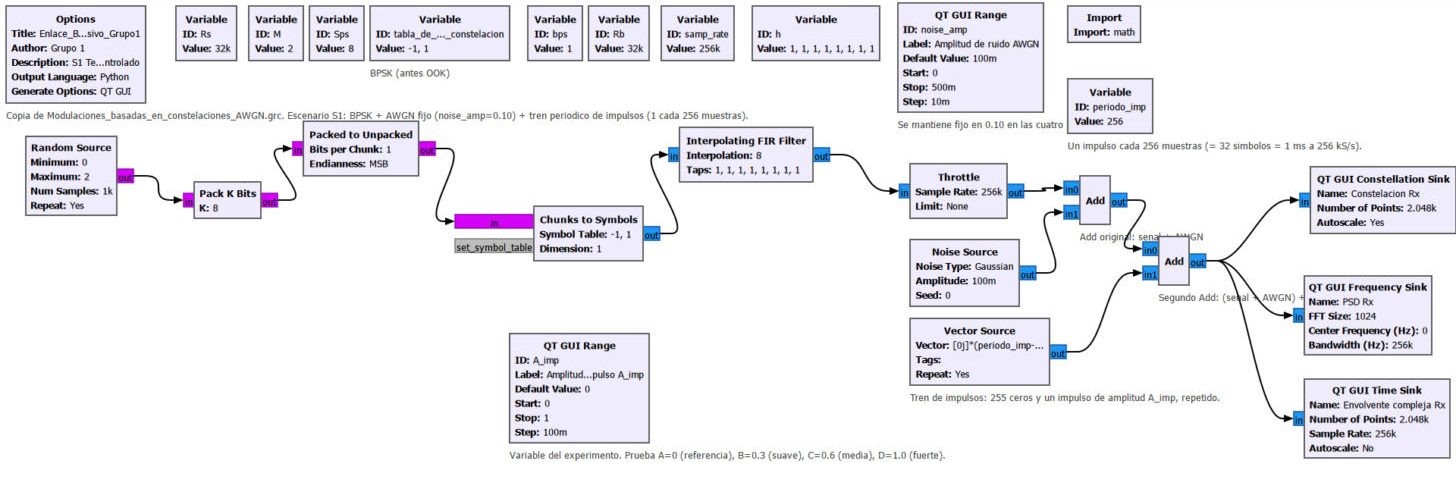
\includegraphics[width=\linewidth]{Figuras/grc_fase1.png}
    \caption{Flujograma de la fase de canal, construido a partir del archivo base del curso: BPSK con pulso rectangular, AWGN de amplitud 0.10 y tren de impulsos de amplitud $A_{imp}$ cada 256 muestras.}
    \label{fig:grc_fase1}
\end{figure}

\subsection{Capturas de GNU Radio por prueba (Fase 2)}
\label{app:capturas}
Las Figs.~\ref{fig:pA}--\ref{fig:pF} reúnen las capturas completas del flujograma de la Fase~2 para cada prueba, siempre con AWGN de amplitud 0.10. En cada figura, a la izquierda está la pestaña \emph{Transmisor y canal} (PSD de la salida del RRC y del canal, envolvente compleja del canal en 8~ms y plano I--Q sobremuestreado) y a la derecha la pestaña \emph{Receptor} (ojo de las componentes I y Q, constelación recuperada y salida del filtro acoplado en 2~ms). La Fig.~\ref{fig:validacion} reúne la pestaña \emph{Validación} de todas las pruebas.

\begin{figure*}[!t]
    \centering
    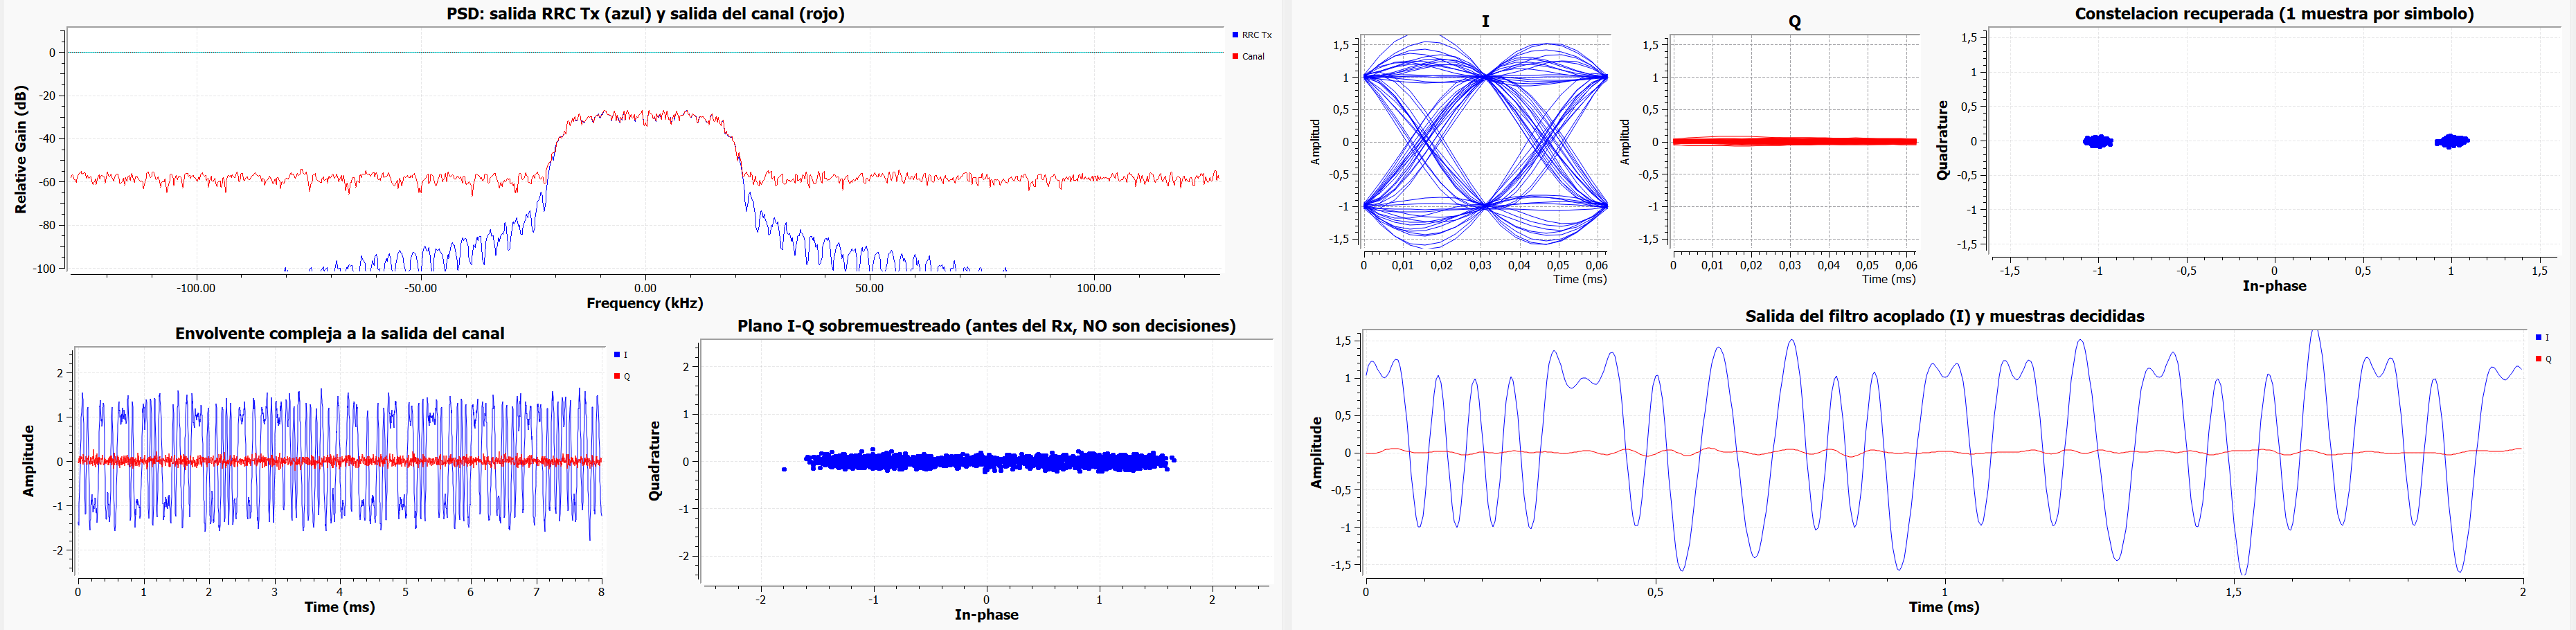
\includegraphics[width=\textwidth]{Figuras/prueba_A.png}
    \caption{Prueba A (referencia, $A_{imp}=0$).}
    \label{fig:pA}
\end{figure*}

\textbf{Prueba A.} Es la línea de base. La PSD del canal reproduce la de la señal RRC dentro de $\pm21.6$~kHz y fuera de ella queda el piso plano del AWGN. La envolvente solo tiene componente I, con niveles alrededor de $\pm1$, y el plano I--Q sobremuestreado es una franja horizontal: son las transiciones entre símbolos, no decisiones. En el receptor, el ojo está abierto por completo y las trayectorias convergen en $\pm1$ en los instantes de muestreo; la constelación recuperada son dos nubes compactas y la componente Q permanece en cero.

\begin{figure*}[!t]
    \centering
    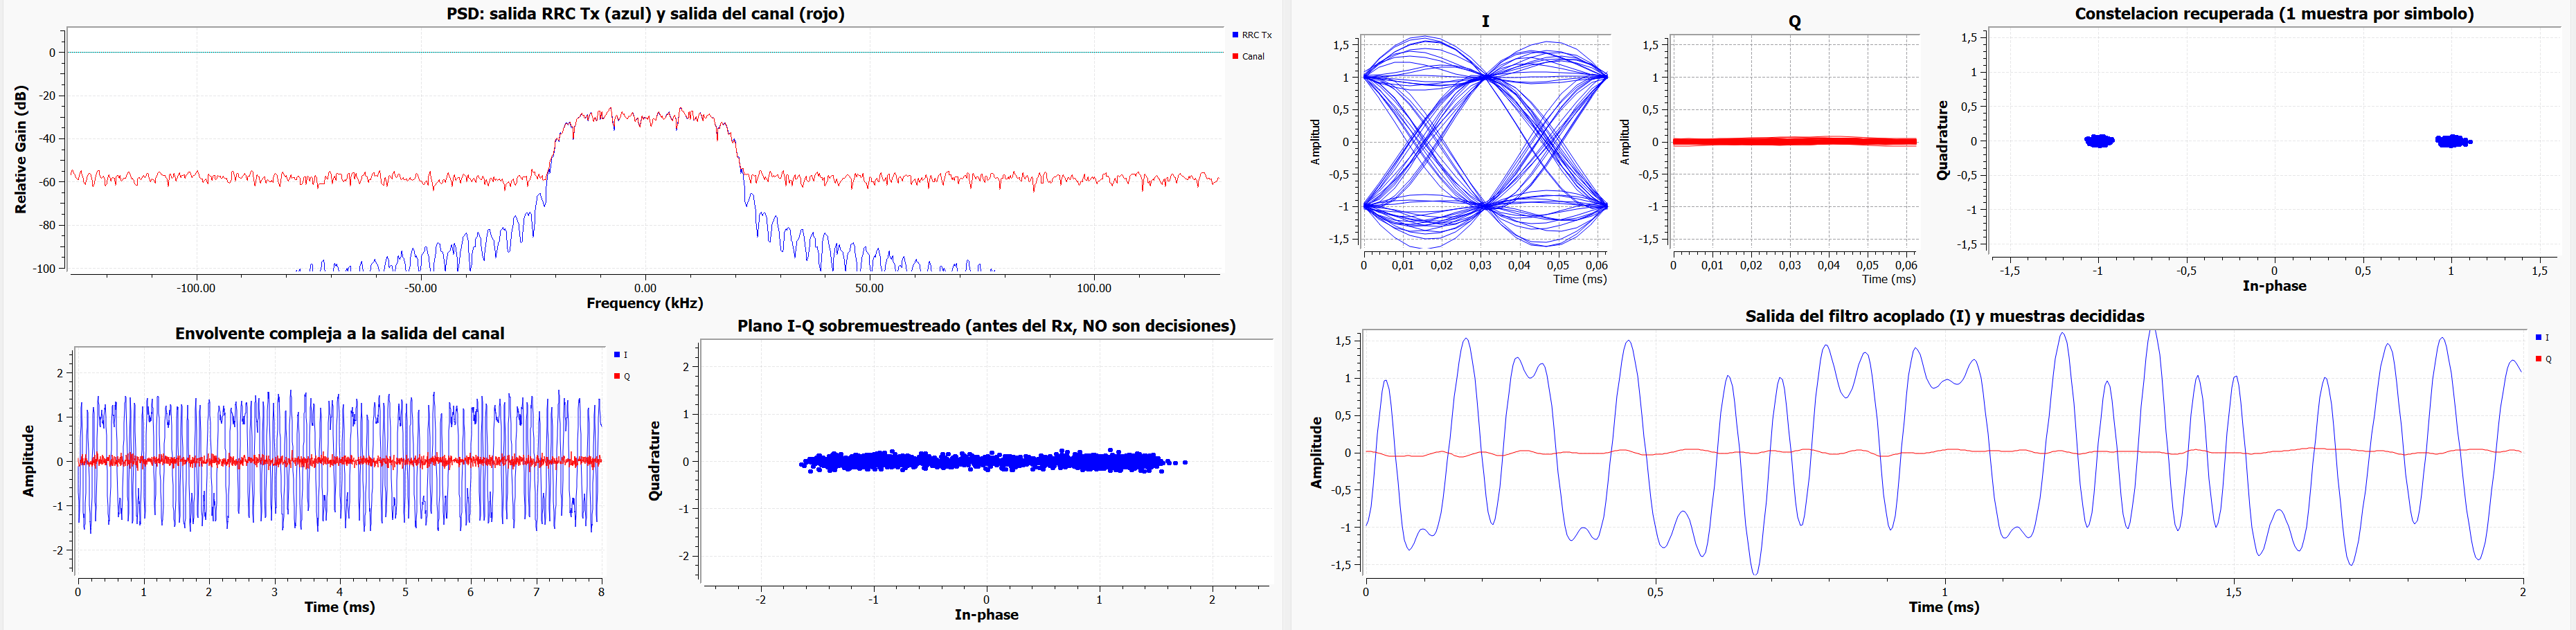
\includegraphics[width=\textwidth]{Figuras/prueba_B.png}
    \caption{Prueba B (perturbación suave, $A_{imp}=0.3$).}
    \label{fig:pB}
\end{figure*}

\textbf{Prueba B.} El tren de impulsos todavía no se distingue en la PSD ni en el ojo. En la envolvente aparecen picos de $\approx1.3$ cada milisegundo cuando el impulso coincide con un nivel positivo. Después del filtro acoplado el impulso se reduce a $0.03$ en la variable de decisión, por eso la constelación es igual a la de la referencia.

\begin{figure*}[!t]
    \centering
    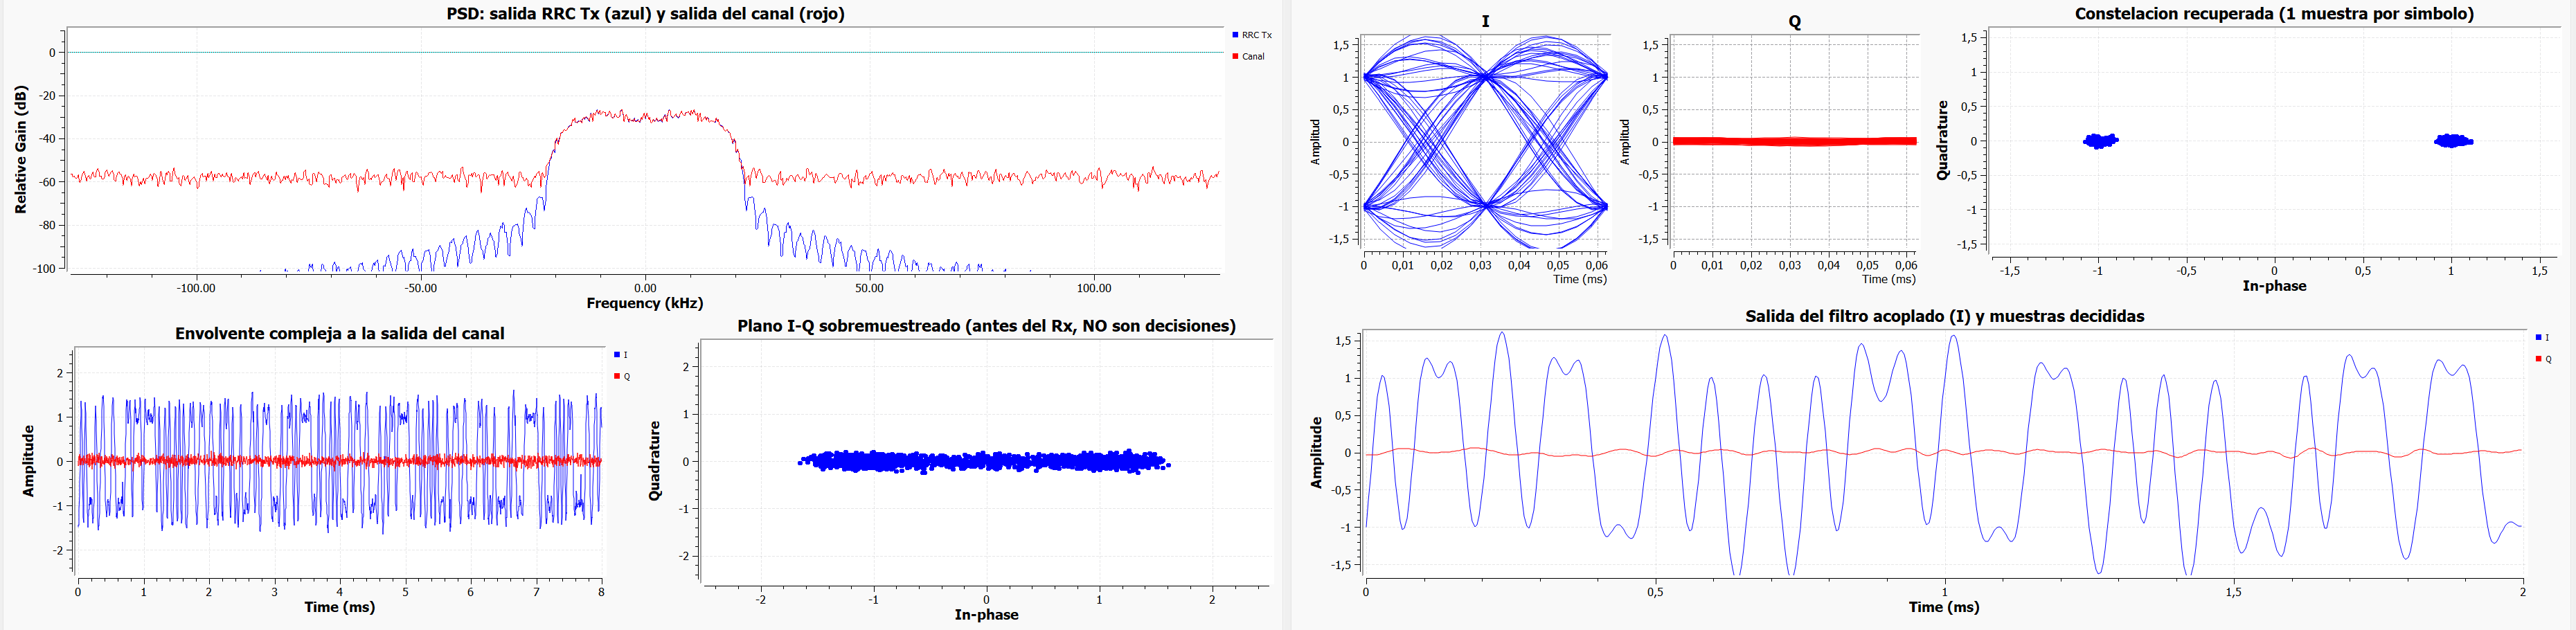
\includegraphics[width=\textwidth]{Figuras/prueba_C.png}
    \caption{Prueba C (perturbación media, $A_{imp}=0.6$).}
    \label{fig:pC}
\end{figure*}

\textbf{Prueba C.} Es la condición principal de análisis. Los picos de la envolvente llegan a $\approx1.6$ y el plano I--Q sobremuestreado se estira ligeramente hacia la derecha. El receptor sigue sin verse afectado: el desplazamiento máximo en la decisión es $0.06$, mucho menor que la distancia de 1 al umbral, y las nubes de la constelación siguen separadas.

\begin{figure*}[!t]
    \centering
    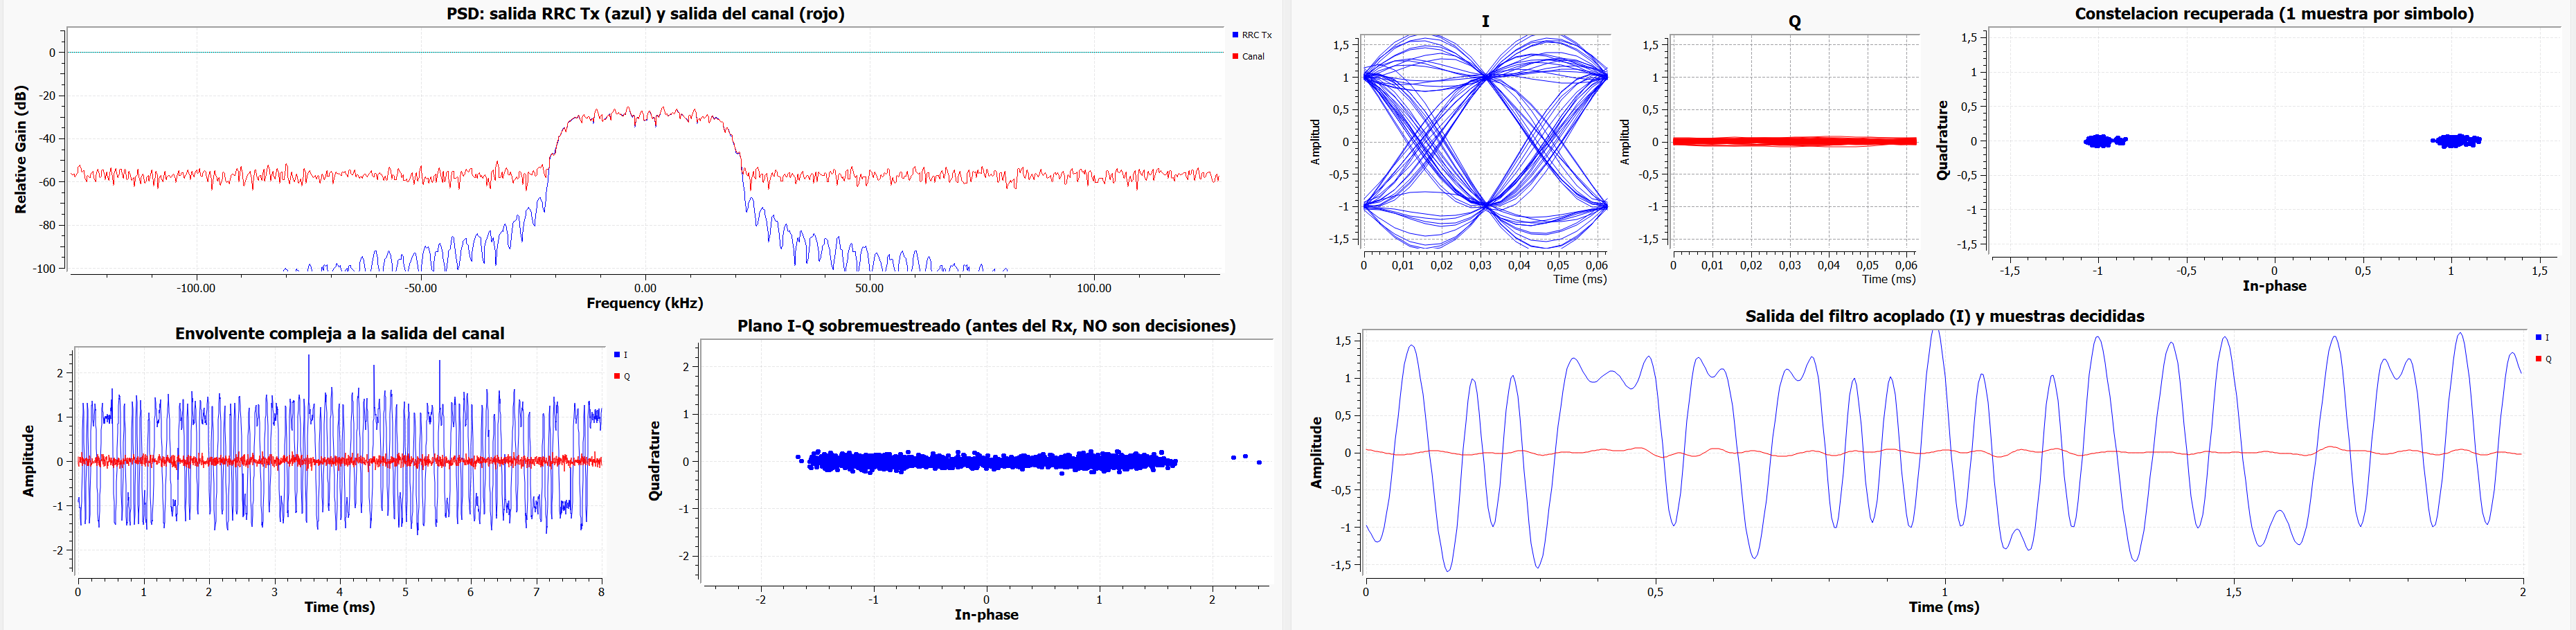
\includegraphics[width=\textwidth]{Figuras/prueba_D.png}
    \caption{Prueba D (perturbación fuerte, $A_{imp}=1.0$).}
    \label{fig:pD}
\end{figure*}

\textbf{Prueba D.} Los impulsos se ven con claridad en el tiempo, con picos que superan 2, y en el plano I--Q aparecen puntos aislados cerca de $I\approx2.3$, fuera de la franja de la señal. En la fase de canal, con pulso rectangular, esta amplitud llevaba los símbolos negativos al umbral. Con el filtro acoplado, la constelación solo muestra unas pocas muestras corridas $\approx0.1$ hacia la derecha y la BER sigue en cero.

\begin{figure*}[!t]
    \centering
    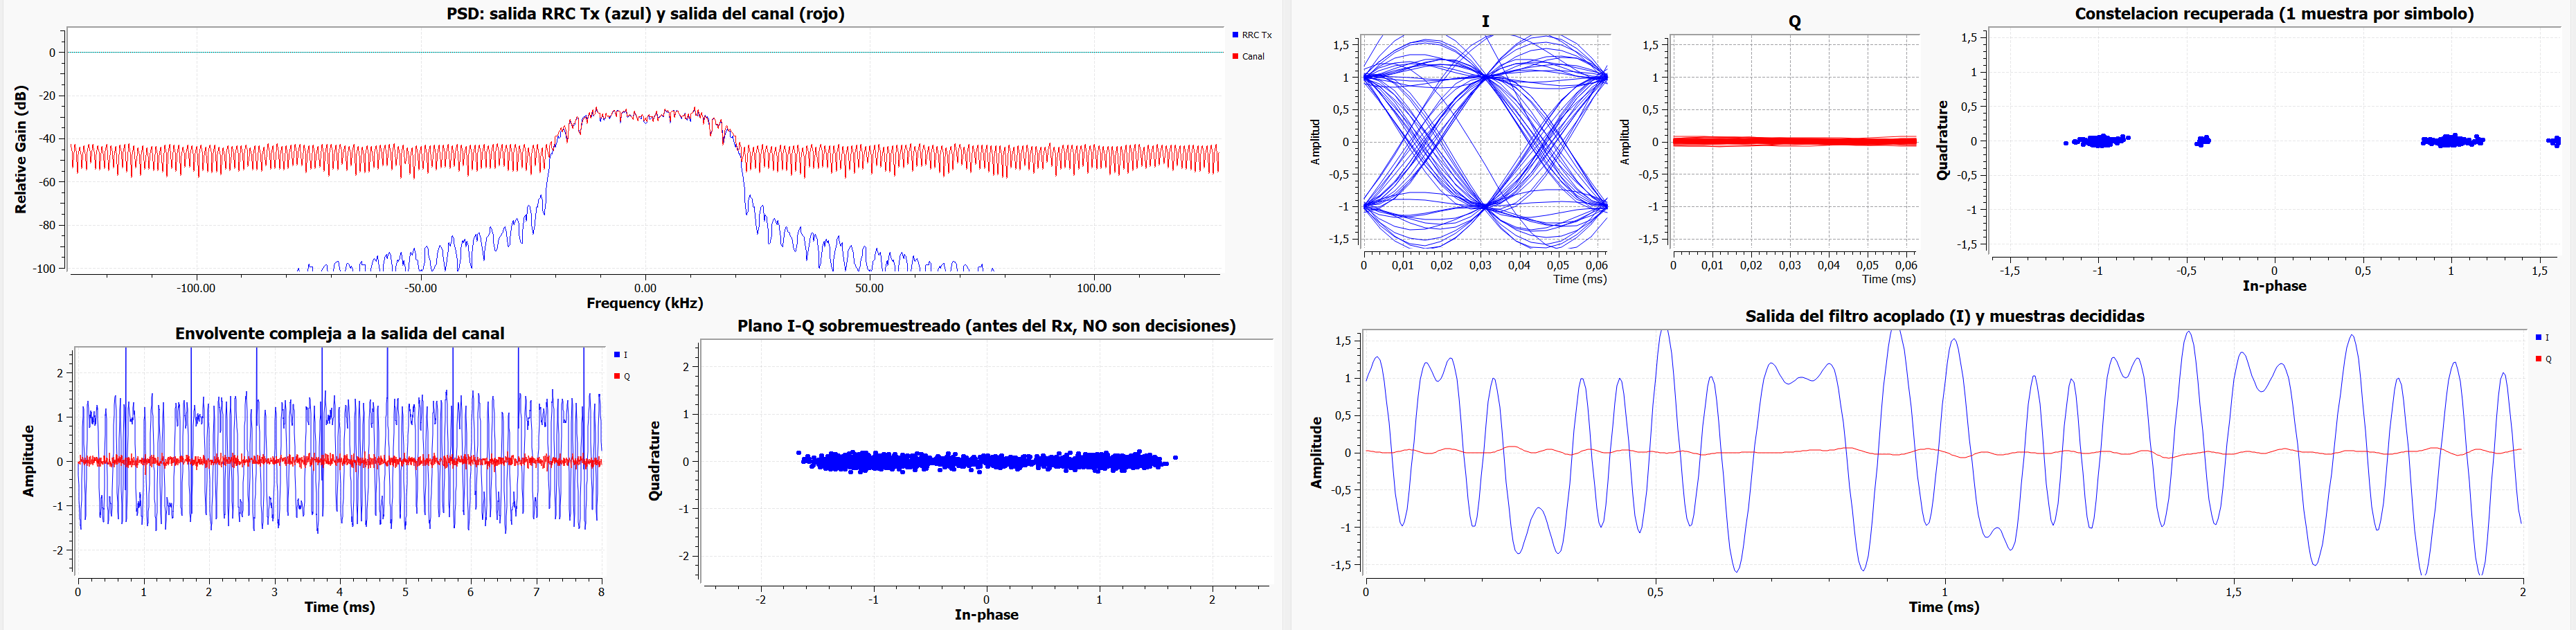
\includegraphics[width=\textwidth]{Figuras/prueba_E.png}
    \caption{Prueba E (robustez, $A_{imp}=5.0$).}
    \label{fig:pE}
\end{figure*}

\textbf{Prueba E.} Con impulsos cinco veces mayores que el símbolo, la PSD sí cambia: el piso sube unos 10~dB y aparece el peine de líneas cada 1~kHz. En la envolvente los picos salen de la escala. En el ojo aparecen trayectorias que se apartan del haz, y en la constelación surgen dos grupos aislados en $-0.5$ y $+1.5$, que son los símbolos que coinciden con un impulso. Aun así ninguna muestra cruza el umbral, porque el margen mínimo es 0.40, y la BER medida sigue en cero.

\begin{figure*}[!t]
    \centering
    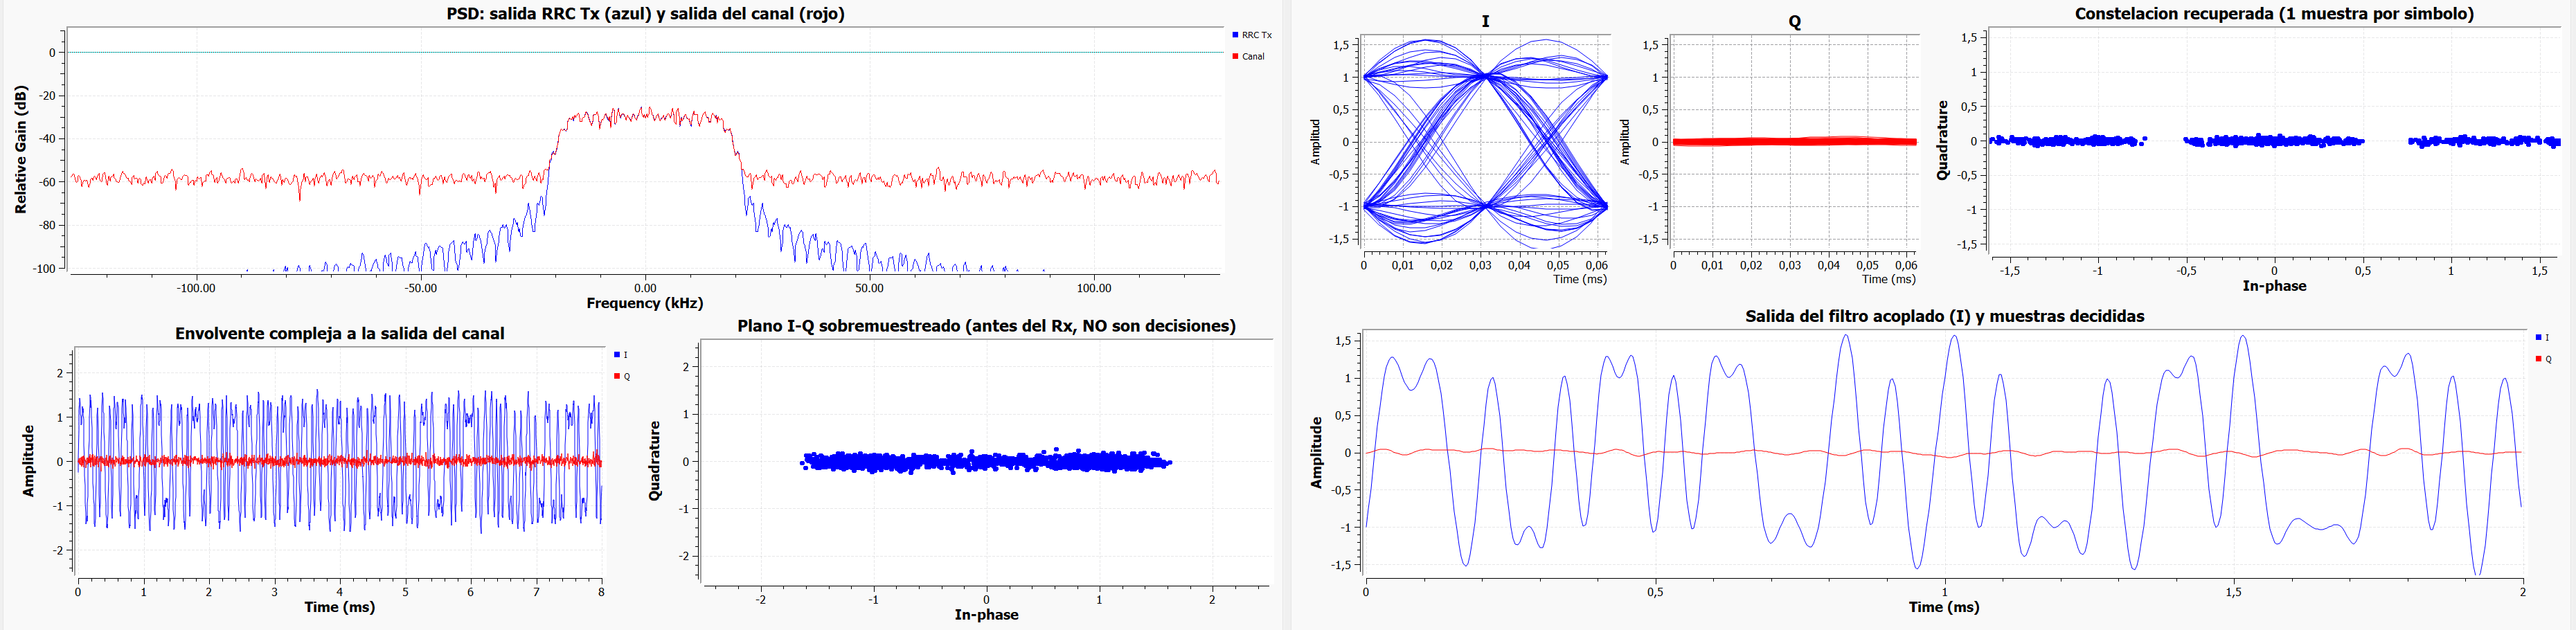
\includegraphics[width=\textwidth]{Figuras/prueba_F.png}
    \caption{Prueba F (referencia muestreada con 4 muestras de desfase).}
    \label{fig:pF}
\end{figure*}

\textbf{Prueba F.} El canal es el mismo de la referencia, como confirma la pestaña izquierda, idéntica a la de la Fig.~\ref{fig:pA}. Lo único que cambia es el instante de muestreo. La salida del filtro acoplado es igual, pero al tomar la muestra en el cruce del ojo la constelación se reparte a lo largo de todo el eje I, con valores cercanos a cero, y la BER sube a 0.2503. Esta prueba muestra que el receptor depende tanto de la sincronización como del canal.

\begin{figure*}[!t]
    \centering
    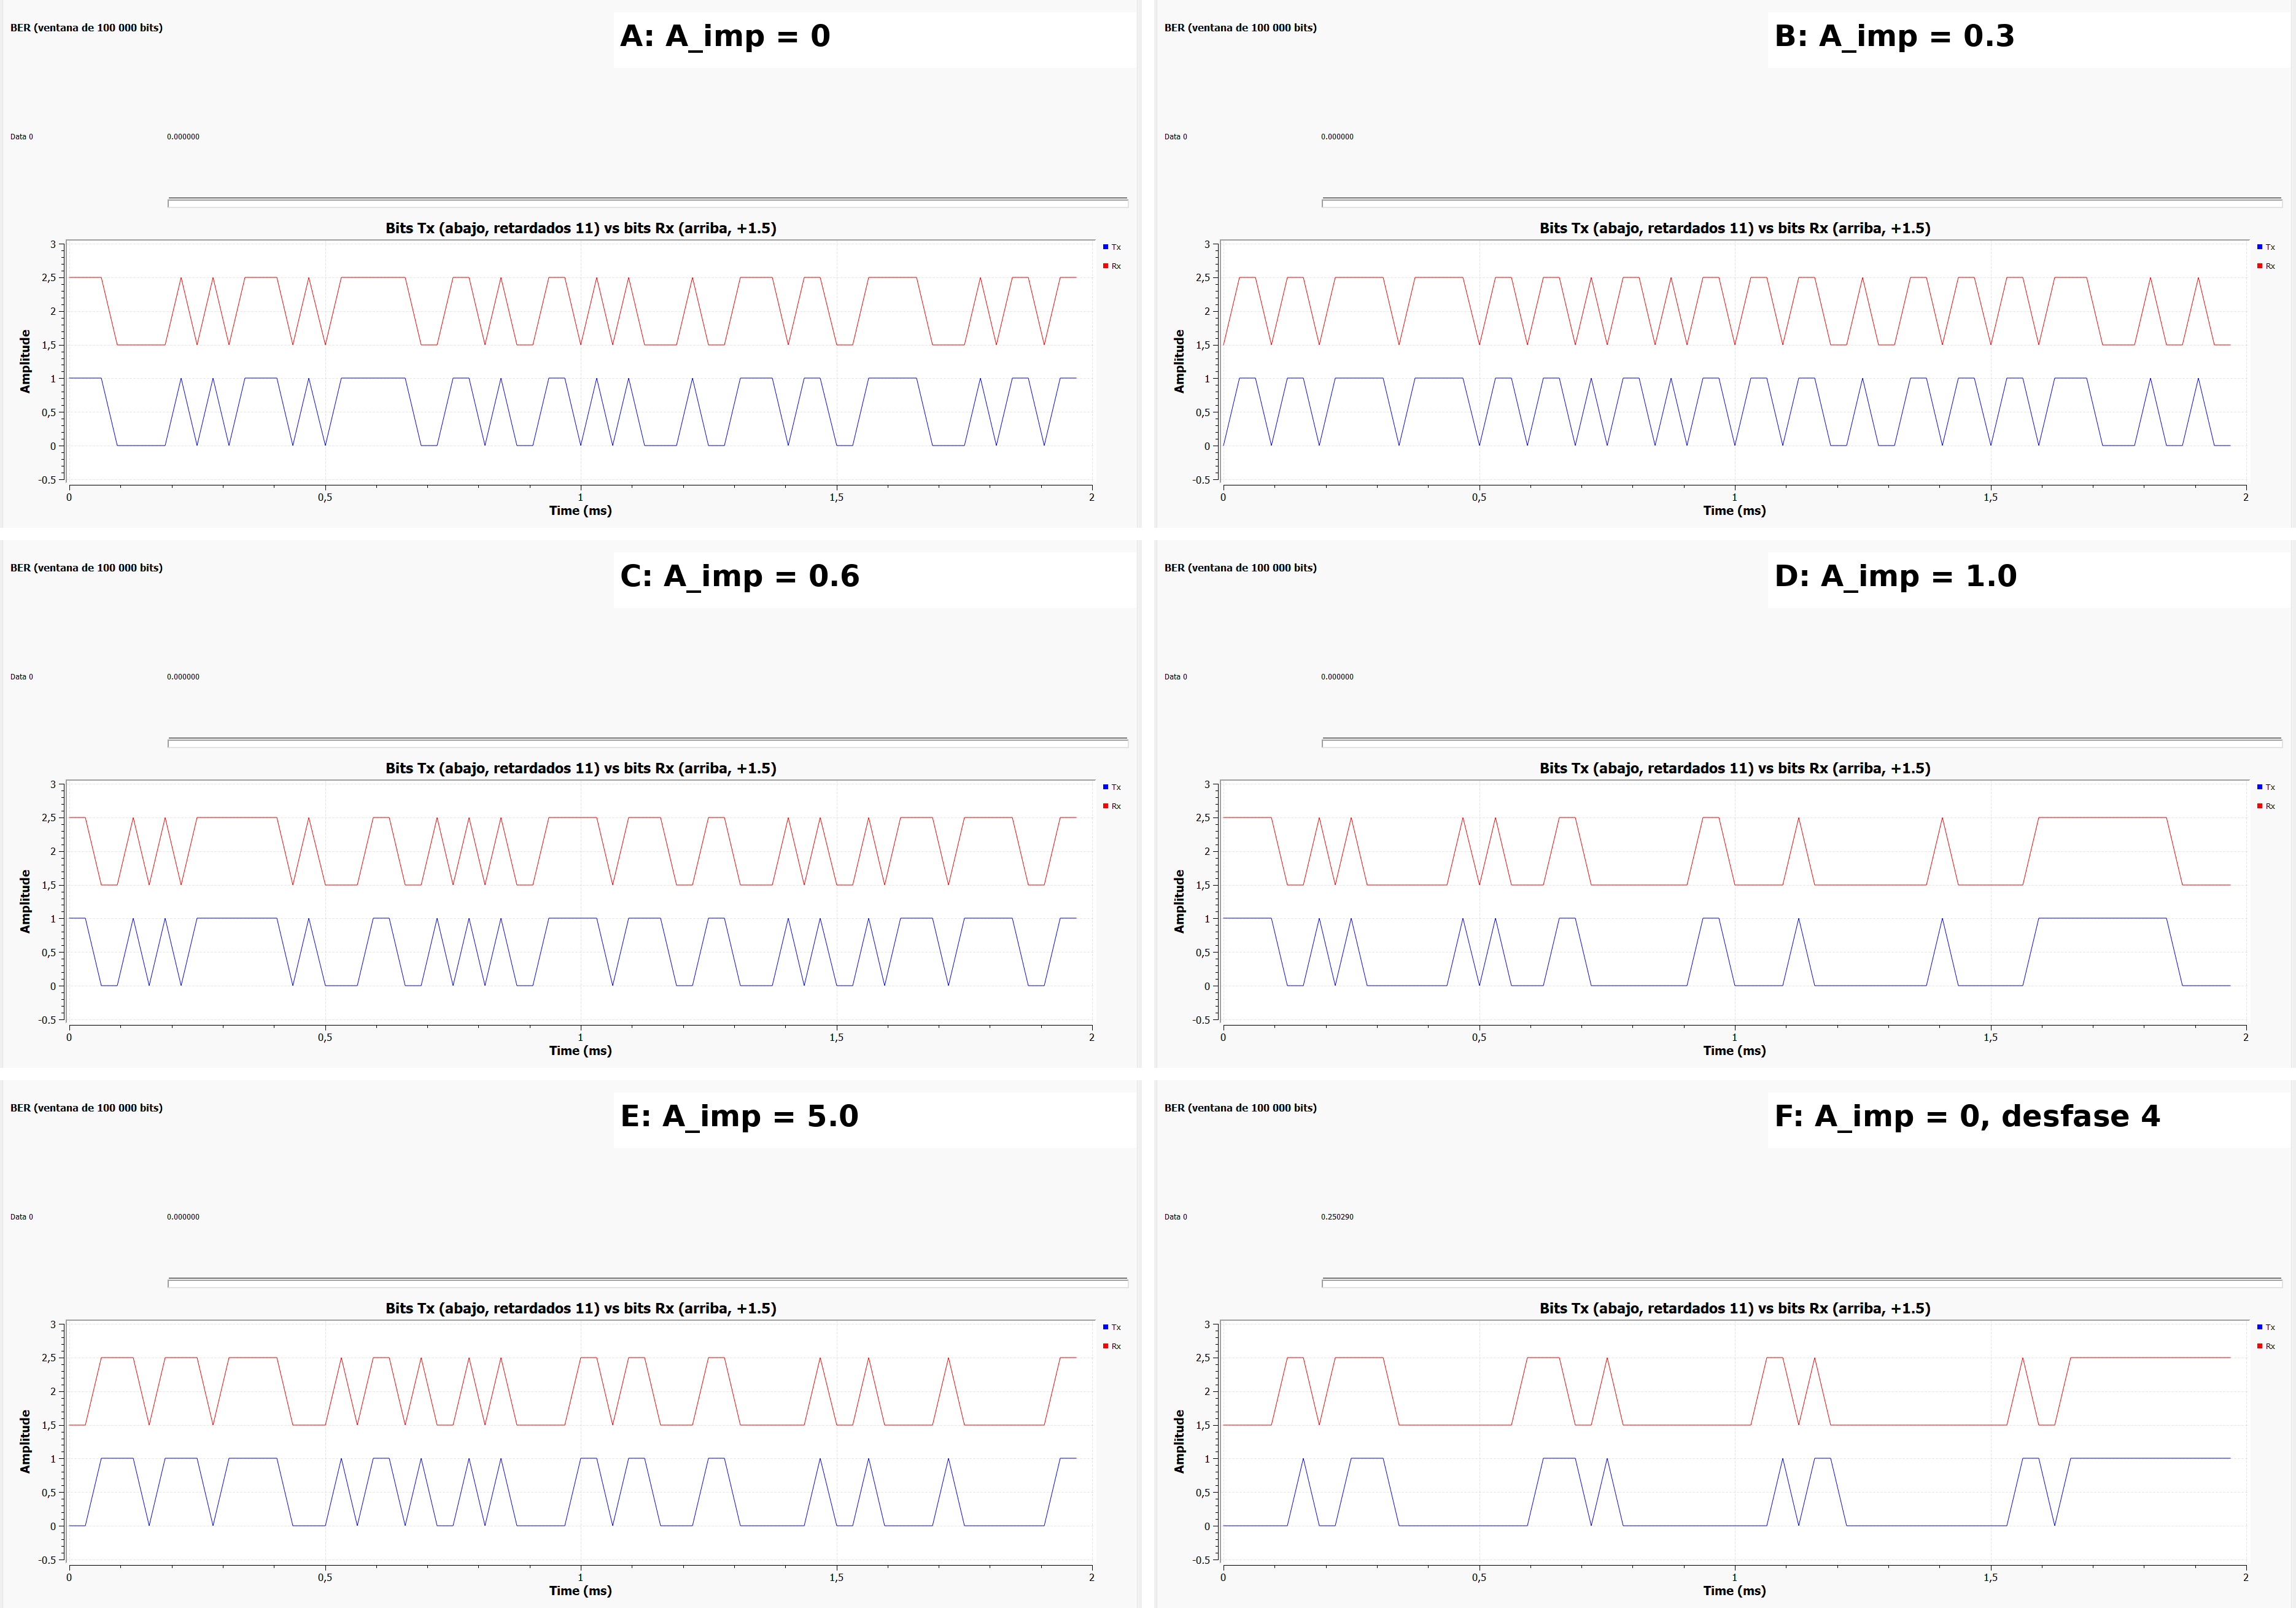
\includegraphics[width=0.92\textwidth]{Figuras/validacion_todas.png}
    \caption{Pestaña \emph{Validación} de las seis pruebas: BER en una ventana de $10^5$ bits y bits transmitidos (abajo, retrasados 11 bits) frente a bits recuperados (arriba, desplazados $+1.5$).}
    \label{fig:validacion}
\end{figure*}
\textbf{Validación.} En las pruebas A a E la BER de la ventana es 0.000000 y las dos secuencias de bits son idénticas, desplazadas solo por el retardo de 11 bits ya compensado. En la prueba F la BER es 0.2503 y se ven bits recuperados que no coinciden con los transmitidos.

\subsection{Ventanas de las curvas BER (Fase 4)}
\label{app:ventanas}
\begin{figure*}[!t]
    \centering
    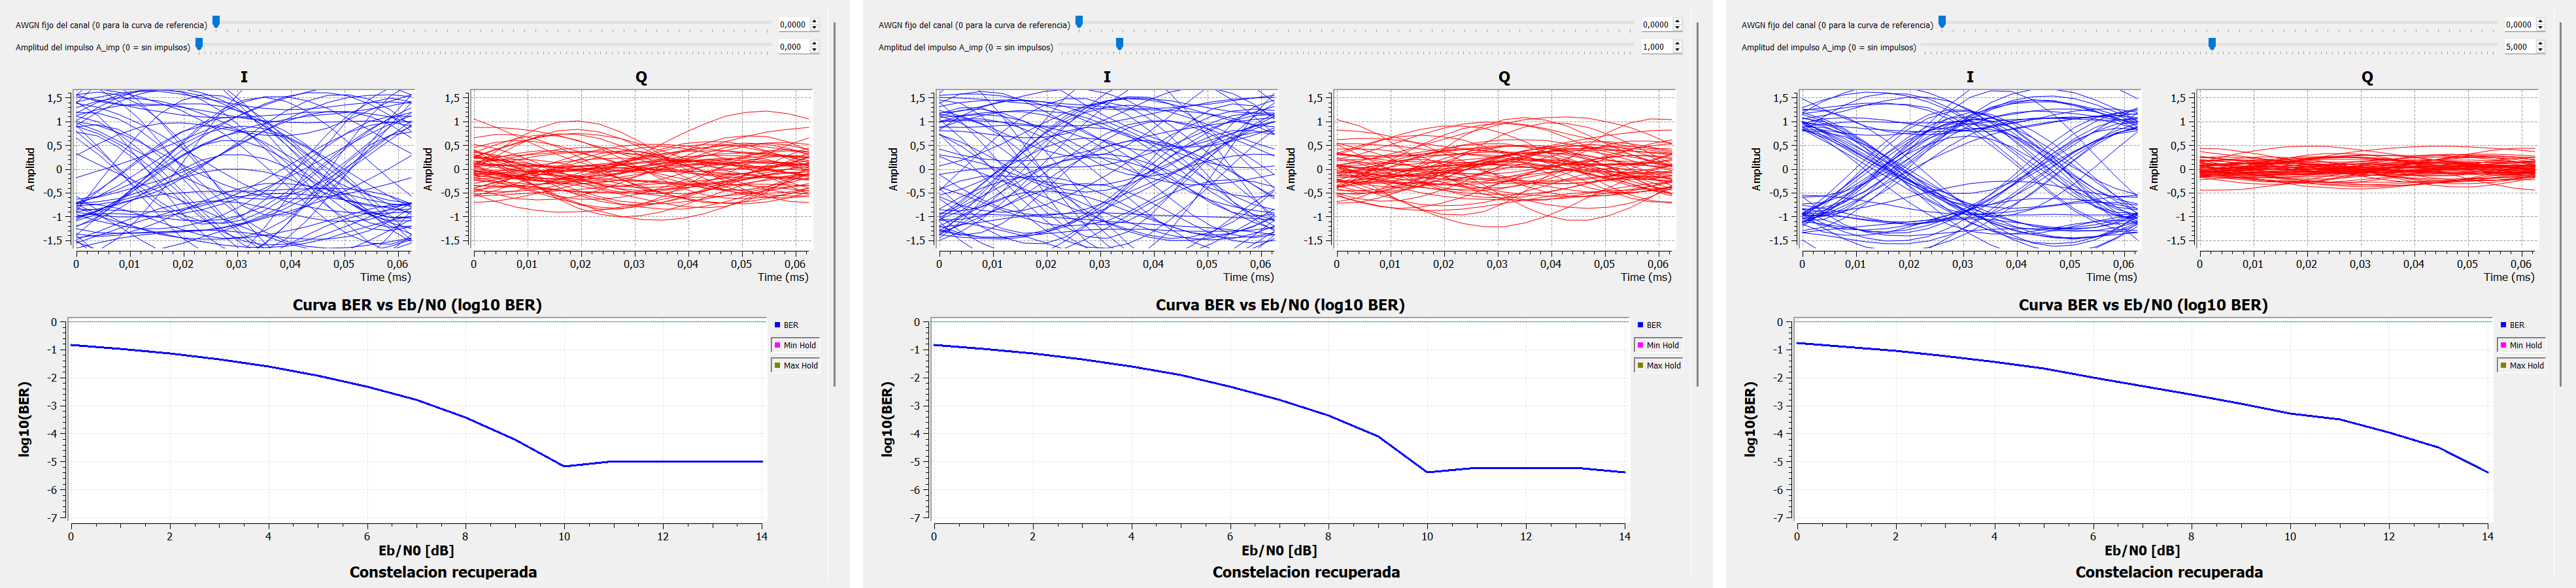
\includegraphics[width=\textwidth]{Figuras/fase4_ventanas.png}
    \caption{Ventanas de los flujogramas de la Fase~4 después de 4 minutos de barrido: sin impulsos (izquierda), $A_{imp}=1$ (centro) y $A_{imp}=5$ (derecha).}
    \label{fig:ventanas}
\end{figure*}
La Fig.~\ref{fig:ventanas} muestra las ventanas de GNU Radio con las que se obtuvieron las curvas de la Fig.~\ref{fig:ber}. El eje vertical es $\log_{10}(\mathrm{BER})$. El ojo de la parte superior corresponde al nivel de ruido del punto del barrido que estaba activo en el momento de la captura, por eso aparece cerrado. En las curvas sin impulsos y con $A_{imp}=1$, el tramo plano a la derecha corresponde a puntos sin errores, que la gráfica dibuja con la cota $3/N$. La curva con $A_{imp}=5$ queda por encima en todo el rango y desciende de forma gradual.

\subsection{Flujograma de medición BER (Fase 4)}
\label{app:fase4}
\begin{figure*}[t]
    \centering
    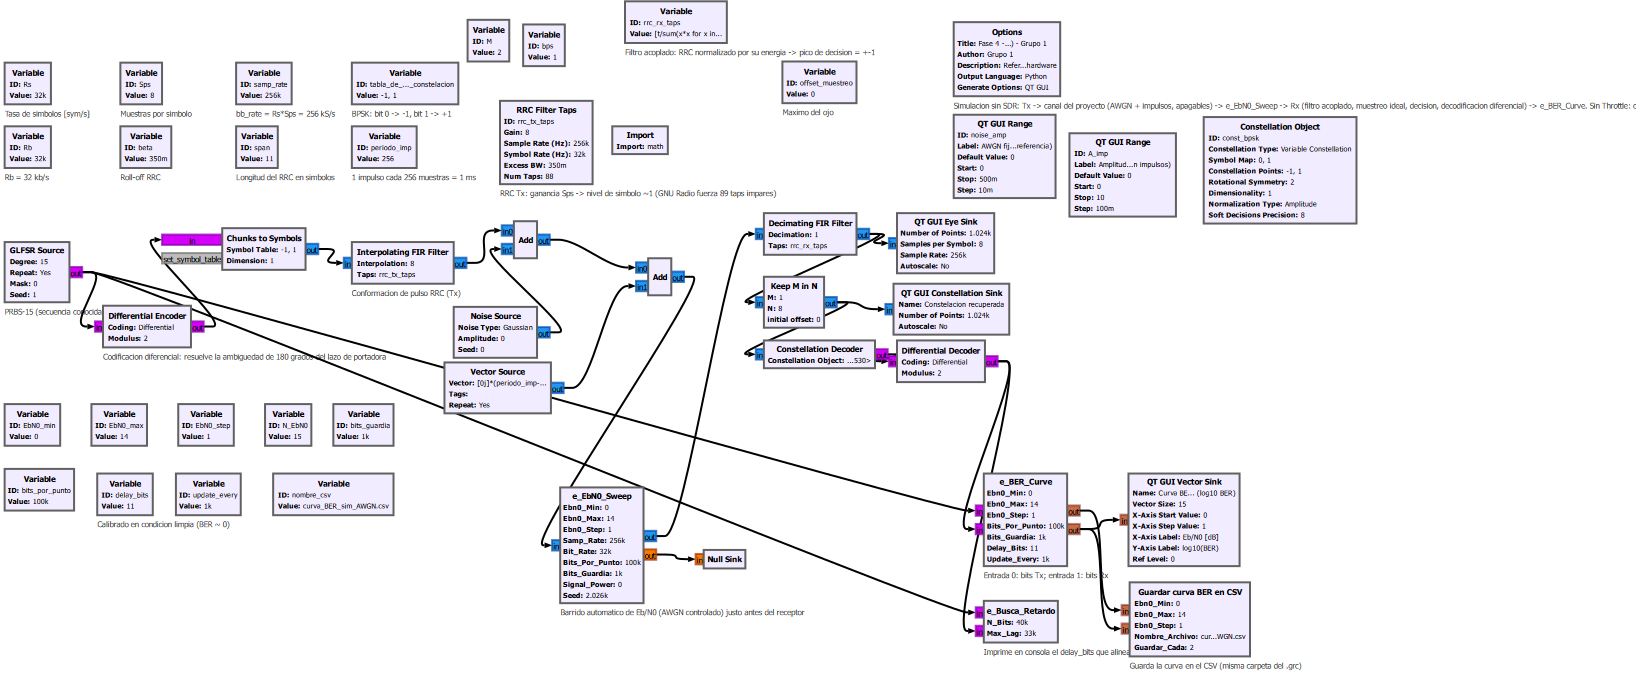
\includegraphics[width=\textwidth]{Figuras/flujograma_fase4.png}
    \caption{Flujograma de medición BER: transmisor con codificación diferencial, canal (AWGN e impulsos), \texttt{e\_EbN0\_Sweep} justo antes del filtro acoplado, receptor (filtro acoplado, muestreo, decisión y decodificación diferencial), \texttt{e\_BER\_Curve} con los bits de la fuente PRBS y los bits recuperados, \texttt{e\_Busca\_Retardo} y el bloque que guarda el CSV.}
    \label{fig:fase4}
\end{figure*}
La Fig.~\ref{fig:fase4} muestra dónde se integró el instrumento. El barrido de ruido se aplica a la señal compleja a 256~kS/s que entra al receptor, y la comparación de bits se hace después de la decodificación diferencial, con la referencia tomada antes del codificador.

\subsection{Evidencias de la práctica de laboratorio}
\label{app:lab}
\begin{figure}[H]
    \centering
    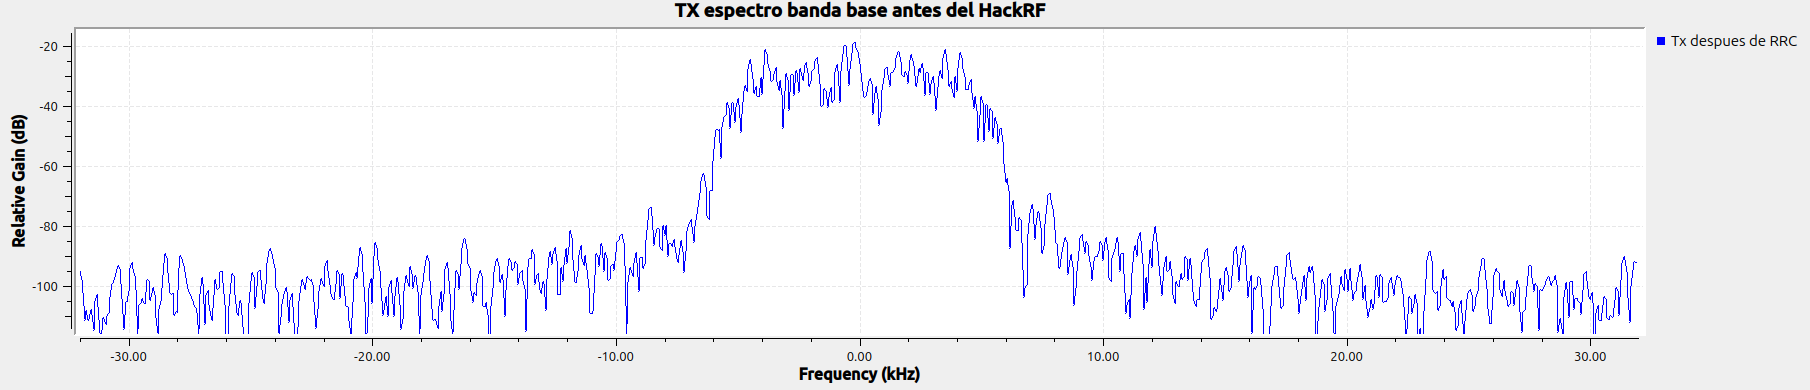
\includegraphics[width=\linewidth]{Figuras/lab_tx_espectro.png}
    \caption{Transmisor HackRF de la práctica de laboratorio: espectro en banda base antes del radio (16-QAM con RRC de roll-off 0.5).}
    \label{fig:lab_tx}
\end{figure}
La Fig.~\ref{fig:lab_tx} muestra el espectro en banda base del transmisor de la práctica. Ocupa unos $\pm6$~kHz, que coinciden con $(1+0.5)\times8$~kHz, y los lóbulos laterales quedan unos 60~dB por debajo.

\begin{figure*}[!t]
    \centering
    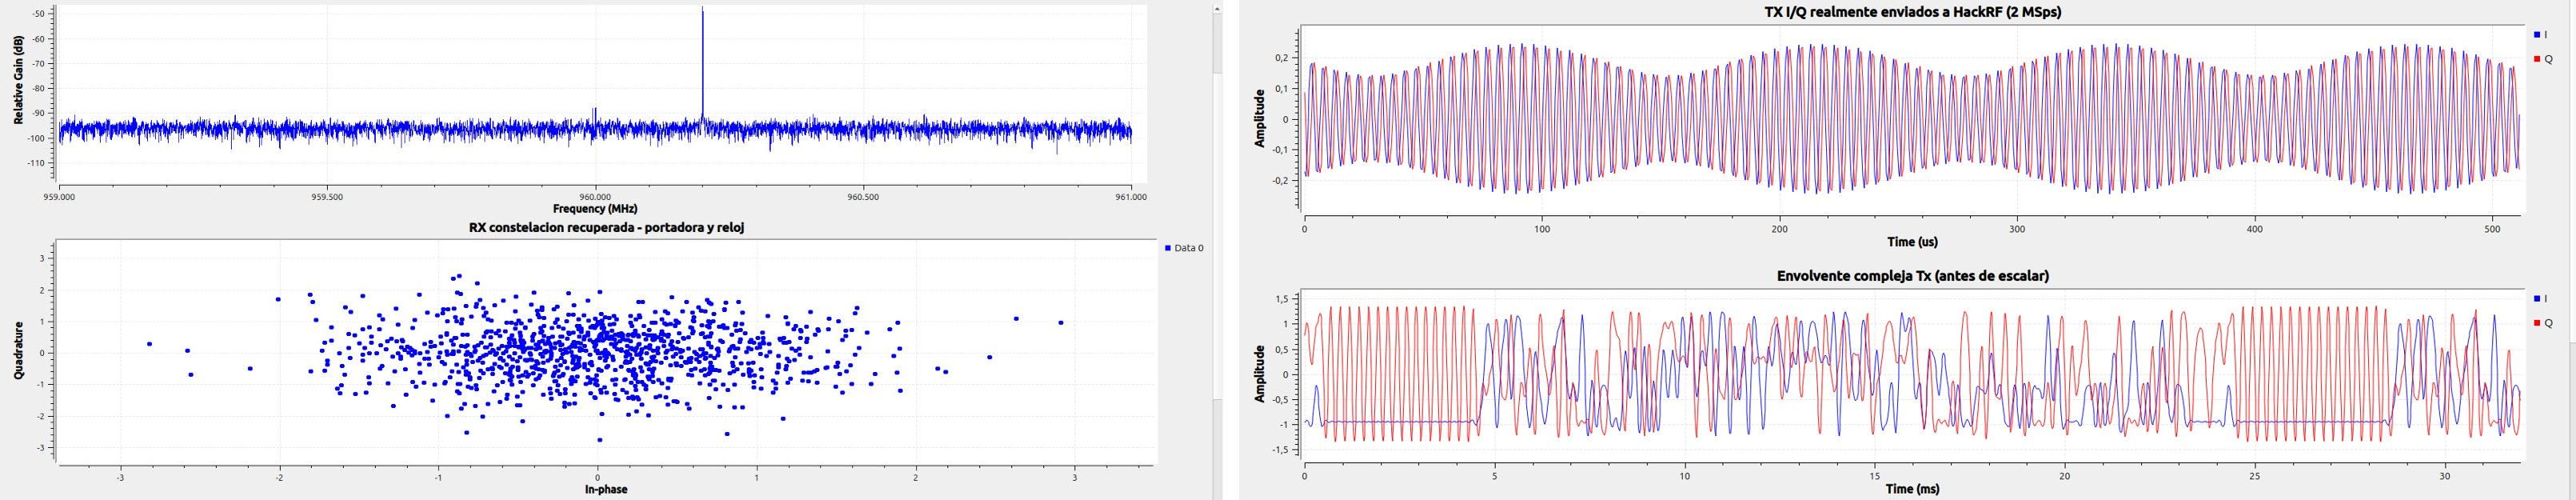
\includegraphics[width=\textwidth]{Figuras/lab_extra.jpg}
    \caption{Práctica de laboratorio. Izquierda: receptor con el transmisor detenido (10:30). Derecha: muestras I/Q enviadas al HackRF (2~MS/s) y envolvente compleja antes de escalar.}
    \label{fig:lab_extra}
\end{figure*}
En la Fig.~\ref{fig:lab_extra}, a la izquierda, sin transmisión el espectro solo conserva la componente de continua del receptor en 960.2~MHz y la constelación se convierte en una nube de ruido centrada en el origen; la amplitud de la salida del filtro baja de $\approx0.1$ a $\approx0.004$. A la derecha, las muestras I/Q realmente enviadas al radio tienen un pico cercano a 0.2, por debajo del límite de 1 del conversor, porque la amplitud digital se fijó en 0.15. Así el transmisor trabaja sin saturar y la potencia se ajusta con la ganancia de RF.

\clearpage
